\documentclass[a4paper,12pt]{article}
\usepackage[osf]{mathpazo}
\usepackage{ms}
\usepackage{natbib}
\usepackage{lineno}
\usepackage{graphicx}
\usepackage{caption}
\modulolinenumbers[5]
\linenumbers

\pdfminorversion=3

\makeatletter
\renewcommand{\@biblabel}[1]{\quad#1.}
\makeatother

\title{How much of the world is woody?}
\author{
Richard G. FitzJohn$^{*,1,2}$, Matthew W. Pennell$^{*,\dag,3,4}$, Amy E. Zanne$^{5,6}$,\\ Peter F. Stevens$^{7,8}$, David C. Tank$^{3,9}$, William K. Cornwell$^{10, 11}$
}
\date{}
\affiliation{\noindent{\footnotesize
$^*$ These authors contributed equally\\
$^\dag$ To whom correspondence should be addressed.\\
$^1$ Biodiversity Research Centre and Department of Zoology,
University of British Columbia, Vancouver, BC V6G 1Z4, Canada
\texttt{fitzjohn@zoology.ubc.ca}\\
$^2$ Department of Biological Sciences, Macquarie University, Sydney, NSW 2109, Australia \\
$^3$ Institute for Bioinformatics and Evolutionary Studies, University
of Idaho, Moscow, ID 83844, U.S.A.
\texttt{mwpennell@gmail.com}\\
$^4$ National Evolutionary Synthesis Center, Durham, NC 27705, U.S.A.\\
$^5$ Department of Biological Sciences, George Washington University,
Washington, D.C. 20052, U.S.A.
\texttt{aezanne@gmail.com}\\
$^6$ Center for Conservation and Sustainable Development, Missouri Botanical Garden, St. Louis, MO, 63121, USA \\
$^7$ Department of Biology, University of Missouri, St. Louis, MO
63166, U.S.A.
\texttt{stevensp@umsl.edu}\\
$^8$ Missouri Botanical Garden, PO Box 299, St Louis, MO 63166-0299\\
$^9$ Department of Forest, Rangeland, and Fire Sciences and Stillinger
Herbarium, College of Natural Resources, University of Idaho, Moscow,
ID 83844, U.S.A.
\texttt{dtank@uidaho.edu}\\
$^{10}$ Department of Systems Ecology, VU University, 1081 HV
Amsterdam, The Netherlands\\
$^{11}$ School of BEES, The University of New South Wales, Sydney 2052 NSW, Australia
\texttt{w.cornwell@unsw.edu.au}}\\

\vfill
% \raggedright, no line numbers, \pagestyle{empty}, copy and paste,
% remove figures (draft mode would be faster) and don't count
% supplement.
% \paragraph{Word-count:} 4179 words
%\paragraph{Manuscript elements:} Fig.~1-3 (bw in print), Appendix.
%\paragraph{Article type:} Note.
}
\runninghead{How much of the world is woody?}
\keywords{Databases, Sampling bias, Macroecology, Herbaceousness, Woodiness, Functional diversity}

\begin{document}
% \raggedright
% \pagestyle{empty}

\mstitlepage
\parindent=1.5em
\addtolength{\parskip}{.3em}

\begin{abstract}
\singlespacing
\begin{enumerate}
\item{
    % RGF: I don't love the first sentence of the abstract (I
    % preferred our original one!).
The question posed by the title of this paper is a basic one, and it is
  surprising that the answer is not known.   A major challenge in the scaling of functional datasets to the global scale is sampling bias.  
  Although we currently know the growth form of many species, these
  data are not a random sample of global diversity;
  some clades are exhaustively characterised, while others we know little--to--nothing about.
  }
  % 
\item{
 Starting with a database of woodiness for 49,064 species of vascular
 plants (17.9\% of taxonomically resolved species, 58\% of which are woody)
  we estimated the status of the remaining taxonomically resolved
  species by randomisation.  
  To compare the results of our method to conventional wisdom, we informally surveyed a broad community of biologists.  No 
  consensus answer to the question existed, with estimates ranging from 1\% to 90\% (mean:
  31.7\%).
}
  %
\item{
 After accounting for sampling bias, we estimated the proportion of woodiness
  among the world's vascular plants to be between 45\% and 48\%.  This was much lower than a simple dataset means and much higher than the conventional wisdom.  
}
  %
\item{
  \emph{Synthesis}: Alongside an understanding of global taxonomic diversity (i.e. number of species globally), building a functional understanding of global diversity is an important new research direction.  This approach represents a new way to account for sampling bias in functional trait datasets and answer basic questions about functional diversity at a global scale.
}
\end{enumerate}
\end{abstract}

\newpage
\doublespacing
\section{Introduction}

The distinction between a woody and non-woody growth-form is
probably the most profound contrast among terrestrial plants and
ecosystems: the difference between a forest and a grassland is the
presence or absence of wood. The recognition of the fundamental
importance of this divide dates back at least to \textit{Enquiry into
  Plants} by Theophrastus of Eresus (371 -- 287 BC), a student of
Plato and Aristotle, who began his investigation into plant form and
function by classifying the hundreds of plants in his garden into
woody and herbaceous categories \citep{theophrastus1916enquiry}.

The last two thousand years of research into wood since Theophrastus
classified his garden have uncovered its origin in the early Devonian
($\sim$~400 Mya; \citealt{gerrienne2011simple}); that prevalence of
woodiness varies with climate \citep{Molesheihgt}; that wood has been
lost many times in diverse groups, both extant and extinct
\citep{judd1994}; and that many different forms of pseudo-woody growth
habit have appeared across groups that have lost true woodiness or
diverged before true woodiness evolved \citep{Cornwellwood}.  We know
about its mechanical properties and developmental pathways, its
patterns of decomposition and their effects on ecosystem function
\citep{Cornwellwood}, and that woody and herbaceous species have
markedly different rates of molecular evolution \citep{SmithDonoghue}.
%
However, we have no idea about what proportion of species in the world
are actually woody.

Functional trait datasets are almost without exception biased.  
Researchers collect data for specific questions on a local scale, and
assembling these local datasets creates a useful resource \citep{kattge2011try}, 
but as with GenBank's assembly of genetic data \citep{smith2011understanding},
the simple compilation of data is not an unbiased sample of global diversity, and 
these biases will in turn bias downstream analyses.
%Possibly refer to the problems caused by bias
Understanding and accounting for the biases in these datasets is a 
important and necessary next step.

We sought to develop an approach that accounts for this bias.  In doing so, we 
were able to re-ask Theophrastus' 2000--year old
question at a global scale: how many of the world's plant species are
woody?
%
We also sought to understand how well scientists were able to overcome this bias and make a reasonable estimate.  To do this 
we took the unconventional approach of coupling our
analysis with with an informal survey in which we asked our question
to the broader community of botanists and other biologists.
% 
%DELETE OR MOVE:
%The tremendous variety of answers in response suggests that at least for this problem overcoming bias requires more than just expert opinion.  
%

\section{Methods and Materials}

\subsection{Dataset}

We use a ``functional'' definition of woodiness; woody species have a
prominent aboveground stem through time, and herbaceous species lack
such a stem \citep[see an early use of this definition
by][]{gray1887elements}.  Note that in addition to species producing
true wood (i.e., consisting of secondary xylem), this definition
classifies, among other groups, palms, tree ferns and bamboo as
woody.
%
We used a recently assembled database with growth--form data for 49,064
vascular plant species (i.e., lycopods, ferns,
gymnosperms and angiosperms), which is the largest such database assembled
to date \citep{Zanne}. 
%
One example of a sub-dataset (6\% of observations in the large dataset) came from Kew Royal Botanic
Gardens dataset on growth form \citep{Kew}.  For the Kew dataset, the
original 103 growth form categories was reduced to a binary
classification.  Fifty-seven of the 103 categories provided enough
information to classify species as either woody or herbaceous
according to our definition (see Table \ref{tab:kew} for specific
decisions).  In addition, many other datasets (collected for a
variety of reasons including forestry inventories) were added
according to the same categorisation \citep{Zanne}.  Like all data
assemblies the component datasets here were collected for a variety of
research goals and have unknown and potentially large sampling biases.

Because the effort to organise plant taxonomy, especially synonymy, is
on-going, there was uncertainty regarding the status of many plant
names.
%
To bring species binomials to a common taxonomy among datasets, names
were matched against accepted names in the Plant List
\citep{ThePlantList}.  Any binomials not found in this list were
matched against the International Plant Name Index
(http://www.ipni.org/) and Tropicos (http://www.tropicos.org/);
potential synonymy in binomials arising from the three lists was
investigated using the Plant List tools \citep{ThePlantList}.  
%
Binomials remaining unmatched were compared first to the Plant List
and if needed to IPNI with an approximate matching algorithm to allow
for misspellings, followed by manual verification.

Theophrastus recognised both the fundamental importance of the
distinction between woody and herbaceous plants, and that this
distinction is in some cases difficult to make.  There are a number of
species which are intermediate (or variable) in form
\citep{beaulieuHiddenRates}; in this dataset 633 species (1.3\%) were
coded as variable and were excluded from our analysis.
%
Our final database contained 37,488 records with both information on
woodiness and documented taxonomy --- 15,657 herbs and 21,831 woody
species.  This included records from all flowering plant orders
currently accepted by APG-III \citep{APG3} and those in the ferns
taxonomy from \citet{apweb}.
% sum(dat.g$K) # known species
% sum(dat.g$H) # herbs
% sum(dat.g$W) # woody species

% WKC: compare family sampling to total number of families? Somehow
% show the dataset is comprehensive?

\subsection{Estimating the percentage of species that are woody}

To estimate the percentage of species that are woody, we cannot simply
use the fraction of species within our trait database (21,831 of
37,488 = 58\%) as these records represent a biased sample of vascular
plants.
% sum(dat.g$W) # woody
% sum(dat.g$K) # known
% sum(dat.g$W) / sum(dat.g$K) # fraction
For example, most Orchidaceae are probably herbaceous; we have only
one record of woodiness among the 1,574 species for which we have
data.
% i.orc <- dat.g$family == "Orchidaceae"
% sum(dat.g$K[i.orc]) # known Orchidaceae
% sum(dat.g$W[i.orc]) # woody Orchidaceae
However, the fraction of Orchidaceae species with known data (1,574 of
27,104 = 6\%)
% sum(dat.g$K[i.orc]) # known Orchidaceae
% sum(dat.g$N[i.orc]) # number of Orchidaceae
% sum(dat.g$K[i.orc]) / sum(dat.g$N[i.orc]) # knowledge rate of Orchidaceae
is much lower than the overall rate of knowledge for all vascular
plants (36,238 of 274,141 = 13\%), which will upwardly bias the global
estimate of woodiness.
% sum(dat.g$K) # known vascular
% sum(dat.g$N) # total vascular
% sum(dat.g$K) / sum(dat.g$N) # knowlege rate for all vascular plants
%
Conversely, systematic under-sampling of tropical species, believed to
be more woody than temperate species \citep{Molesheihgt}, would bias
the global woodiness estimate downwards.

%WKC: After doing all that annoying dataset checking for Amy's paper
%I figured out where the bias is from:  there are several forestry datasets 
% of exclusively woody species that got pulled in.  So basically in the tropics, esp. the paleo-tropics
% various British people were trying to figure out what makes good wood to build the buildings of the british 
% empire so they 
% did a rather systemtic inventory of woody properties of the local species
% since 

We developed a novel method to account for this sampling bias when
estimating the percentage of woody species.  In our approach, we treat
each genus separately, and in all cases know that there are are $n_w$
woody and $n_h$ species and a total of $N$ species in the genus.
%
For example, the genus \textit{Microcoelia} (Orchidaceae) has 30
species in total, and we know that 13 are herbaceous and none are
known to be woody ($N = 30$, $n_w = 0$, $n_h = 13$). We do not know
the state of the remaining 17 species, so the true number of woody
species, $N_w$, must lie between 0 and 17. In general, we cannot
assume that these species are all herbaceous, even though both
biological and mathematical intuition suggest that most of them will
be.

We used two different approaches for imputing the values of these
unknown species. First, we assumed that the known species were sampled
without replacement from a pool of species with $N_w$ woody and $N_h$
herbaceous species ($N_w + N_h = N$), following a hypergeometric
distribution. The probability that $x$ of the species of unknown state
are woody ($x = 0, 1, \ldots, N - n_w - n_h$) is proportional to
\begin{equation}
  \Pr(N_w = x) \propto {n_w + x \choose n_w}
  {N - n_w - x \choose n_h}
\end{equation}
For \textit{Microcoelia} this gives a 45\% probability that all
species are herbaceous, and a 92\% chance that at most three species
are woody.

This approach probably overestimates the number of woody species in
this case, and in other cases where all known species are woody (e.g.,
\textit{Actinidia} [Ericaceae]) it will probably underestimate the
number of species that are woody. We see this as corresponding to a
very weak prior on the shape of the distribution of the fraction of
woody species within a genus.

However, the distribution of woodiness among genera and families is
strongly bimodal; most genera are either all-woody or all-herbaceous
(Figure \ref{fig:distribution-genera} and 
\citealt{sinnott1915evolution}).  Among the 748 genera with at least 10
records, 392 are entirely woody, 248 are entirely herbaceous, and only
50 have between 10\% and 90\% woody species. As a result, knowing the
state of a handful of species within a genus can give a reasonable
guess at the remaining species.
% tmp <- dat.g$p[dat.g$K >= 10] # genera with 10 records
% sum(tmp == 1) # 100% woody
% sum(tmp == 0) # 100% herbaceous
To model the other extreme of sampling, we used an approach where we
computed the observed fraction of woody species ($p_w = n_w / (n_w +
n_h)$) and sampled the state of the unobserved species using a
binomial distribution, so that the probability that $x$ of the species
are woody is
\begin{equation}
  \Pr(x = k) = {N - n_w - n_h \choose k - n_w} 
  p^k (1-p)^{N - n_h - k}.
\end{equation}

In cases where all known species are woody (or herbaceous) this will
assign all unknown species to be woody (or herbaceous). In polymorphic
cases this will give similar results to the hypergeometric sampling
approach above. This approach corresponds to a very strong prior on
the shape of the distribution of woodiness among genera.
While neither of these approaches is ``correct'', they probably
span the range of possible outcomes.

For genera where there was no information on woodiness for any
species, we sampled a fraction of species that might be woody from the
empirical distribution of woodiness fractions \textit{among genera}
within the same order. We did this after imputing the missing species
values within those other genera. So, if a genus is found in an order
with genera that had woodiness fractions of $\{0, 0, 0.1, 1\}$ we would
have approximately a 50\% chance of sampling a 0\% woodiness fraction
for a genus, with probabilities from 0.1 to 1 being fairly evenly
spread.  Given this woodiness fraction, we then sampled the number of
species that are woody from a binomial distribution with this fraction
and the number of species in the genus as its parameters.

\subsection{Survey}

% The idea is that the above shows how our biological data sets are
% biased vs the actual data (as in, we've collected the information in
% a biased way).
%
% The point of the survey is that not only are we not aware of the
% bias, but our *guesses* as to what the mean actually is is also
% biased.
In estimating the number of species within Angiosperm families,
\citet{joppa2010} found that expert opinion generally agreed closely
with estimates from a statistical model.  We were interested in
whether a consensus answer existed --- even if not formalised in the
literature --- and if so, whether it was consistent with the data.
% 
We created an English-language survey (which we also translated into
Portuguese) asking for an estimate of the percentage of species that
are woody according to the above definition.  We also asked
respondents to indicate their level of familiarity with plants, level
of formal training, and the country in which they received their
training. We sent out the survey to several internet mailing lists and
social media websites (see Appendix and Supplementary Figure
\ref{fig:survey-text} for details on the survey).

\section{Results}

Across all vascular plants, we estimated the fraction of woody species
to be between 45\% to 48\%.
% round(100*res.strong$overall, 1)
% round(100*res.weak$overall, 1)
Specifically, using our ``strong prior'' sampling approach we
estimated 45.0\% of species are woody (95\% confidence interval of
44.7--45.3\%) and with the ``weak prior'' approach we estimated 47.2\%
(95\% CI of 46.6--47.8\%).
% mean(d.survey$Estimate < 45)
% mean(d.survey$Estimate < 100*res.strong$overall[["mean"]])
The different approaches generate different distributions of the
per-genus percentage of woodiness (Figure
\ref{fig:distribution-genera}), with a less strongly bimodal
distribution using the ``weak prior'' approach.  However, the two different approaches (strong
versus weak priors) led to similar phylogenetic distributions of
estimated woodiness (Figure \ref{fig:phylogeny} versus Figure
\ref{fig:phylogeny-supp}), differing only in detail.

%
Because the observed distribution of woodiness fraction among genera
is itself strongly bimodal, we believe that the true result lies
closer to 45\% than to 47\%.  A more sophisticated hierarchical
modelling approach could lead to a more precise answer, but we feel
that our values probably span the range of estimates that such an
approach would generate.

There was strikingly little consensus among researchers as to the
percentage of species that are woody.  We received 292 responses from
28 countries, with estimates that ranged from 1\% to 90\% with a mean
of 31.7\% (Figure \ref{fig:survey-distribution}).  Our smallest
estimate is greater than 81\% of our survey estimates.
% nrow(d.survey)
% range(d.survey$Estimate)
% mean(d.survey$Estimate)
We found little effect of a respondent's level of training on their
estimate (Figure \ref{fig:survey}).  There was a significant effect of
the respondent's familiarity with plants on the estimates, primarily
driven by respondents with little botanical familiarity (the ``What's
a Plant?'' category), whose estimates tended to be lower (less woody)
than the estimates from other categories.
%
Before carrying out the survey, we had hypothesised that researchers
from tropical regions may perceive the world as woodier than
researchers from more temperate regions due to the latitudinal
gradient in woodiness \citep{Molesheihgt}.
%
Indeed, there was an effect of being in a tropical country, with the
estimates from tropical countries being slightly higher than those
from temperate countries ($p$=0.02), but this effect was very small
($r^2$=0.02, Figure \ref{fig:survey-distribution}).




\section{Discussion}

% No consensus
Our estimates of woodiness differed from both the survey and the
simple mean of the global database: neither simple statistics nor
expert intuition were accurate in this case.  The difference from
expert knowledge is in striking contrast to \citet{joppa2010}, who
found that that expert opinion on the number of species within
different Angiosperm groups agreed closely with results based on
analyses of data and their bias.
%Surprisingly, there was no consensus of opinion as to how woody the
%world is.  We find it very surprising that this most basic aspect of
%plant natural history was not generally known.  
%Fewer woody that we thought
The respondents to the survey perceived there to be substantially fewer woody
species in the world than there probably are.  This herb--centric view
of the world may arise from the importance of our (mostly herbaceous)
cultivated crops, or the fact that people --- including researchers
--- likely spend more time in the garden than in the forest, especially in tropical forests where most diversity lies.

%
%less woody than the database mean
Our estimate of the percentage of species that are woody (45--47\%)
differs from the raw estimate based on species in our database (58\%).
This difference is caused by the interaction between biased sampling
and clustered trait data at a variety of taxonomic scales.
%
The distribution of woodiness is bimodal among genera, and the
distribution of sizes of those genera differs with woodiness.  Genera
that are primarily herbaceous (less than 10\% woody species for genera
with at least 10 records) were on average larger than primarily woody
genera (more than 90\% woody species), with a mean of 202 species
compared to 138.  This means that even a random sampling above the
level of species will lead to a biased estimate.

%Effects of sampling bias
The effect of selection bias on the estimate is amplified by the distribution of woodiness at higher
taxonomic levels, with families or even orders often being
predominantly either woody or herbaceous (Figure \ref{fig:phylogeny} and
\citealt{sinnott1915evolution}).  There are two major clades that are
primarily herbaceous --- the monocots and ferns
(Monilophyta). However, there are many primarily herbaceous clades
nested within woody clades, and vice versa, which makes the
combination of taxonomic and functional information crucial for
answering this type of question.  

Higher--order classifications are at least as much a product of human
pattern matching as biological processes.  Genera correspond to the
morphological discontinuities among species that humans deem important
\citep{scotland2004significance}, which likely includes woodiness
\citep[e.g.,][]{Hutchinson}.  The relative rarity of genera with
significant numbers of both woody and herbaceous species (Figure
\ref{fig:distribution-genera}) reinforces the importance of this
trait.  A significant, but unaccounted for, source of error is the likely
nonrandom woodiness of undiscovered species.  In principle,
rarefaction analysis could estimate the number of species remaining to
be discovered in different groups, but this is not possible for many
plant clades \citep{costello2011}.

While we have focused on one trait, sampling biases are pervasive in ecological datasets, and need to be addressed.
Global databases of functional traits
\citep[e.g., TRY;][]{kattge2011try} are central to biodiversity
research, but through no fault of database collator they are inevitably biased in terms of taxonomic breadth
and this may have serious consequences for the reliability of
inferences drawn from them.
For example, for woodiness the economic importance of forestry species
likely leads to their
over-sampling in this dataset.
This bias also affects many commonly used methods in ecological and evolutionary research \citep[e.g.,][]{ackerly2000taxon,nakagawa2008missing,pennell2013integrative} in addition to its well understood effects on conventional statistics.  In this case, taking the data at face--value, 
we would have greatly overestimated
the global percentage of woody species.  Inferring the global
frequency of any trait would face the same problem.  For
example, the ecologically important traits of nitrogen--fixing,
mycorrhizal symbioses and pollinator syndrome are strongly
taxonomically structured, and we would expect raw estimates to be
biased in the same way as woodiness was.  Our approach was developed
for binary traits
but similar approaches could be developed for multi--state categorical or continuous traits.

The availability of global databases for genetic and functional traits is one of the recent key developments in ecology and evolutionary research.  These databases have the promise of allowing researchers to address broad--reaching and long--standing questions by drawing on huge amounts of accumulated research.  
Just as Theophrastus' garden was a non-random sample of the Greek
flora, our trait databases contain diverse biases; accounting for
them will be important in making inferences about broad-scale
ecological and evolutionary patterns and processes.

\section{Acknowledgements}

We thank the members of the Tempo and Mode of Plant Trait
Evolution working group for contributing to project development,
members of the broader community who took the time to fill out and
comment on our survey and Rafael Maia for translating our survey and
helping us to distribute it.  In particular, thank we Jon Eastman for 
developing the taxonomic resources we used for this study.
%
We thank Dales Indian Cuisine in Durham, NC for providing the buffet
lunch over which this project was brought to life.
%
This work was supported by the National Evolutionary Synthesis Center
(NESCent), NSF \#EF- 0905606, Macquarie University Genes to Geoscience
Research Centre through the working group.
%
RGF was supported by a Vanier Commonwealth Graduate Scholarship from
the Natural Sciences and Engineering Research Council of Canada
(NSERC).
MWP was supported by a NESCent graduate fellowship and a 
University of Idaho Bioinformatics and Computational Biology graduate fellowship.
%
WKC was supported by Netherlands Organisation for
Scientific Research (NWO) through its Open Competition Program of the
section Earth and Life Sciences (ALW) grant nr. 820.01.016.

\section{Appendix: Survey details}
%
The survey we created is included as a Supplementary Figure to
this paper (see \ref{fig:survey-text}). We distributed the survey to the 
community via several electronic
mailing lists with wide circulation among biologists: \emph{EvolDir},
\emph{ECOLOG}, \emph{\mbox{r-sig-phylo}}, \emph{Taxacom},
\emph{Herbaria}, as well as local lists. We also posted links on the
social-networking platforms \textsc{google+}, \textsc{twitter} and
\textsc{facebook} to reach a broad audience.
%
In order to increase representation of survey responses from Latin
America, we translated the survey into Portuguese and distributed it
to Brazilian biology \textsc{facebook} groups and university mailing
lists.

To analyse the survey data, we used linear regression on
logit-transformed percent woodiness as \citep[see][]{wartonarcsine}
and treated the self-reported level of botanical familiarity and
education as factors.  We converted country of training to coarse
latitude using shapefiles
from the GBIF dataportal\\
(\texttt{http://code.google.com/p/gbif-dataportal/wiki/ConfiguringGeoserver}),
and converted these into ``tropical'' and ``temperate'' using an
absolute latitude of 23$^\circ$~26$^\prime$.  All analyses were
conducted with R version 2.15.1 \citep{R}.


\bibliographystyle{jecol}
\bibliography{wood.bib}

\begin{figure}[p]
  \centering
  \includegraphics{figs/fraction-by-genus}
  \caption{Distribution of the percentage of woodiness among genera.
    The distribution of the percentage of species that are woody within
    a genus is strongly bimodal among genera (panel A -- showing
    genera with at least 10 species only).
    % 
    The two different sampling approaches generate distributions that
    differ in their bimodality (panel B). When assuming species are
    sampled with replacement from some pool, but having no prior on
    the fraction of woodiness within the pool generates a broad
    distribution with many polymorphic genera (blue lines), while
    sampling with replacement assuming that species are drawn from a
    pool of species that has a fraction of woody species equal to the
    observed fraction of woodiness generates a strongly bimodal
    distribution (red lines).}
  \label{fig:distribution-genera}
\end{figure}

\begin{figure}[p]
  \centering
  \includegraphics{figs/fraction-on-phylogeny}
  \caption{Distribution of the percentage of woodiness among orders of
    vascular plants.  Each tip represents an order, with the width of
    the sector proportional to the square root of the number of
    recognised species in that order (data from accepted names in
    \citet{ThePlantList}).  The bars around the perimeter indicate the
    percentage of woody (brown) and herbaceous (green) species,
    estimated using the ``strong prior'' (sampling without
    replacement) approach.  Using the ``weak prior'' approach
    generally leads to an estimated percentage that is closer to 50\%
    (see Figures \ref{fig:phylogeny-supp} and
    \ref{fig:distribution-genera}).  Phylogeny from \citep{Zanne}.
    Orders not placed by APG-III \citep{APG3} are not displayed.}
\label{fig:phylogeny}
\end{figure}


\begin{figure}[p]
  \centering
  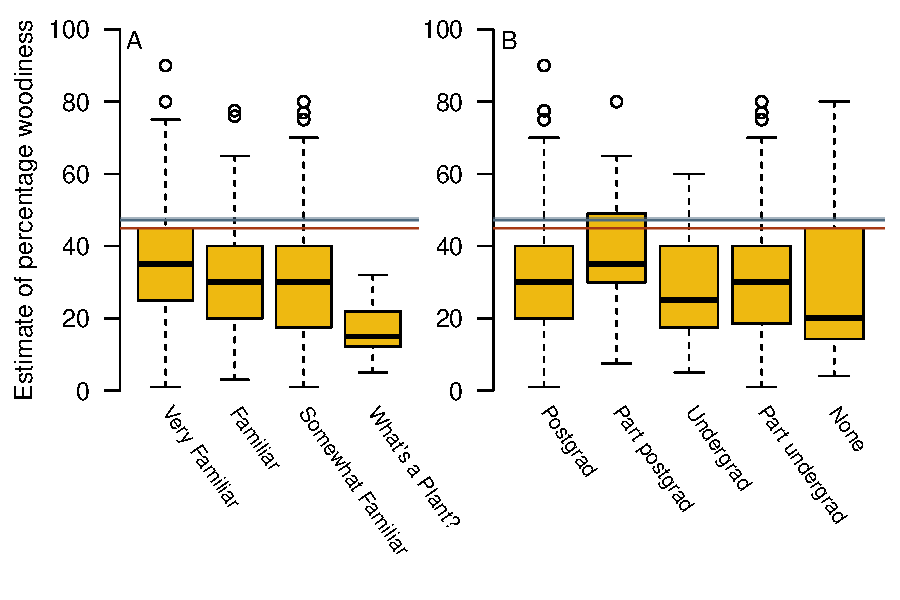
\includegraphics{figs/survey-results}
  \caption{Distribution of responses to the survey question ``What
    percentage of the world's vascular plant species are
    woody?''. Responses are broken up by familiarity with plants
    (panel A) and formal training in botany or a related discipline
    (panel B). The mean and 95\% confidence intervals for our
    estimates of the proportion of woody species from the empirical
    data are depicted by the horizontal shaded rectangles; the blue
    upper rectangle corresponds to the ``weak prior'' approach and the
    red lower rectangle corresponds to the ``strong prior'' approach
    (see Appendix for details).}
  \label{fig:survey}
\end{figure}

\clearpage
\renewcommand\thefigure{S.\arabic{figure}}
\renewcommand\thetable{S.\arabic{table}}
\setcounter{figure}{0}    
\setcounter{table}{0}    

\begin{figure}[p]
  \centering
  \vspace{-20ex}
  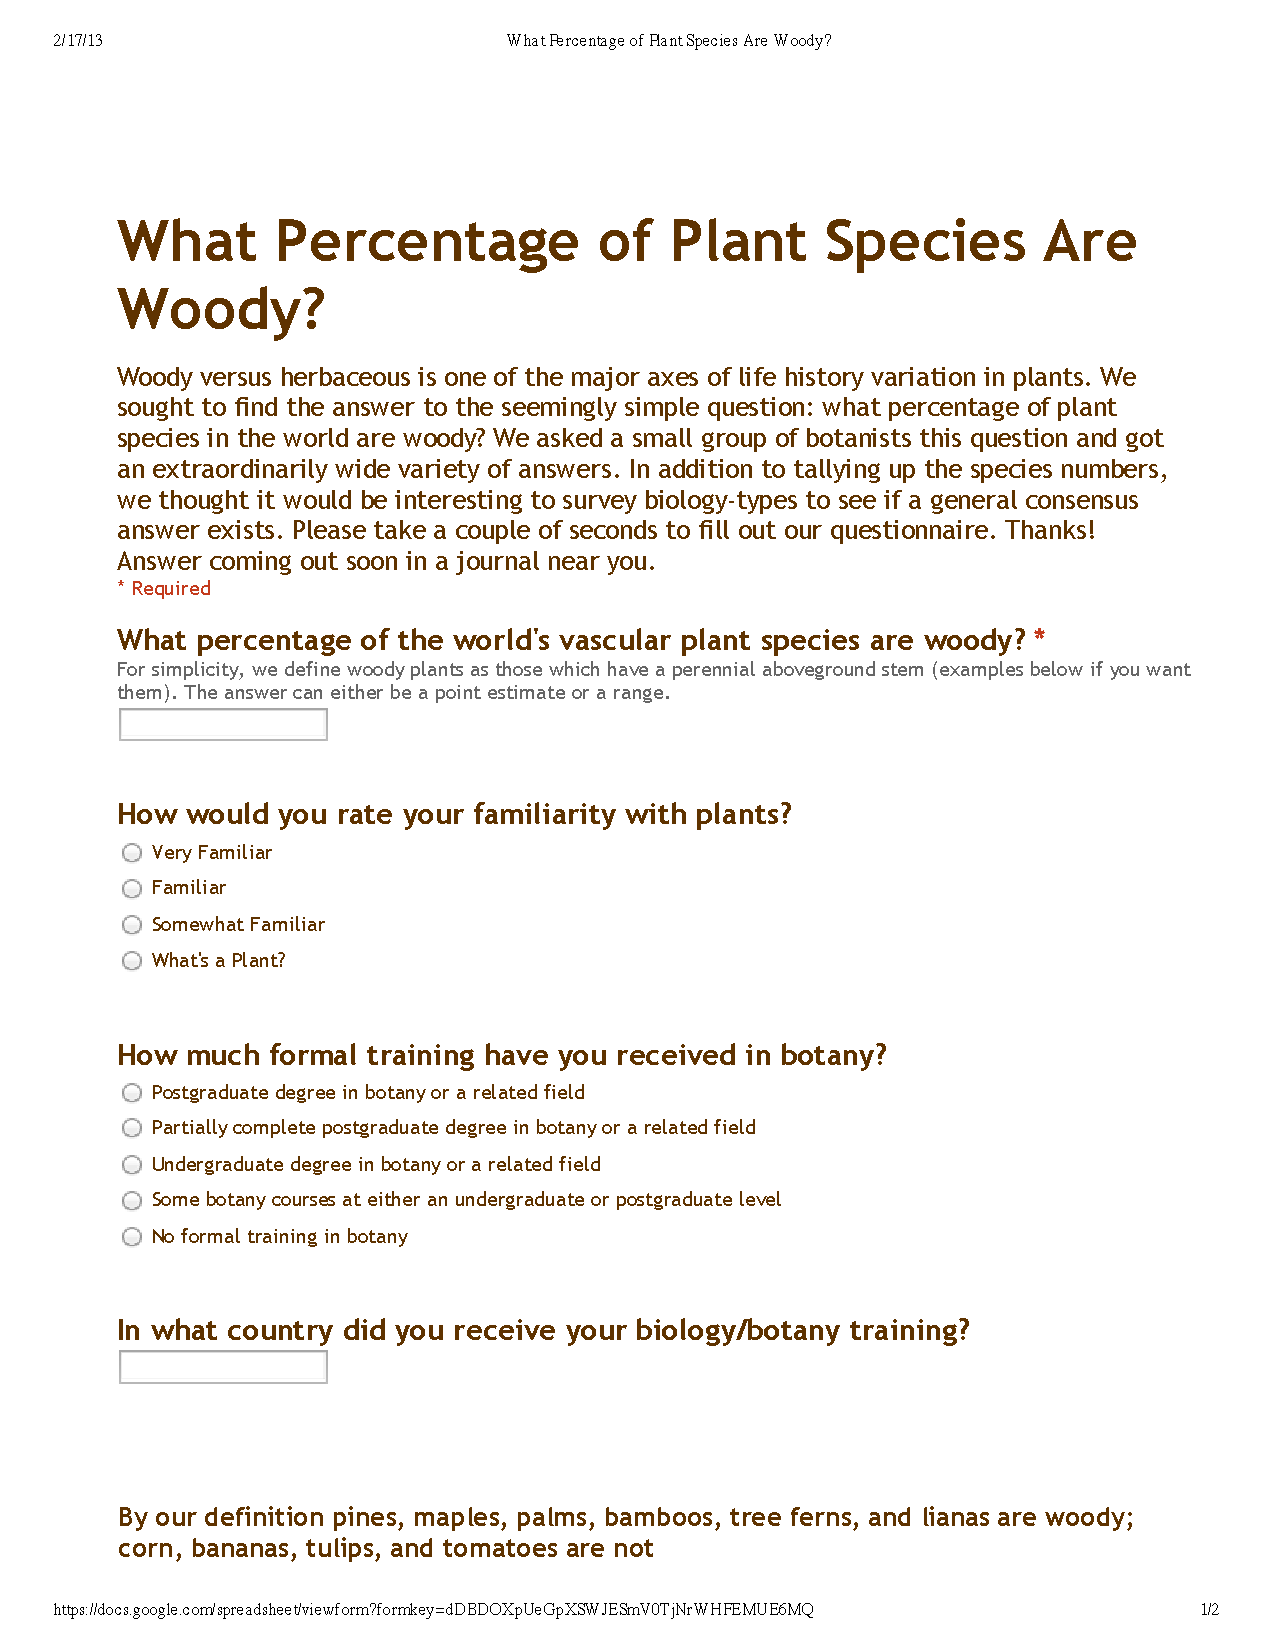
\includegraphics[scale=0.7]{figs/Survey_supplemental}
  \caption{(Supplementary) English-language version of the survey we
    distributed}
  \label{fig:survey-text}
\end{figure}

\begin{figure}[p]
  \centering
  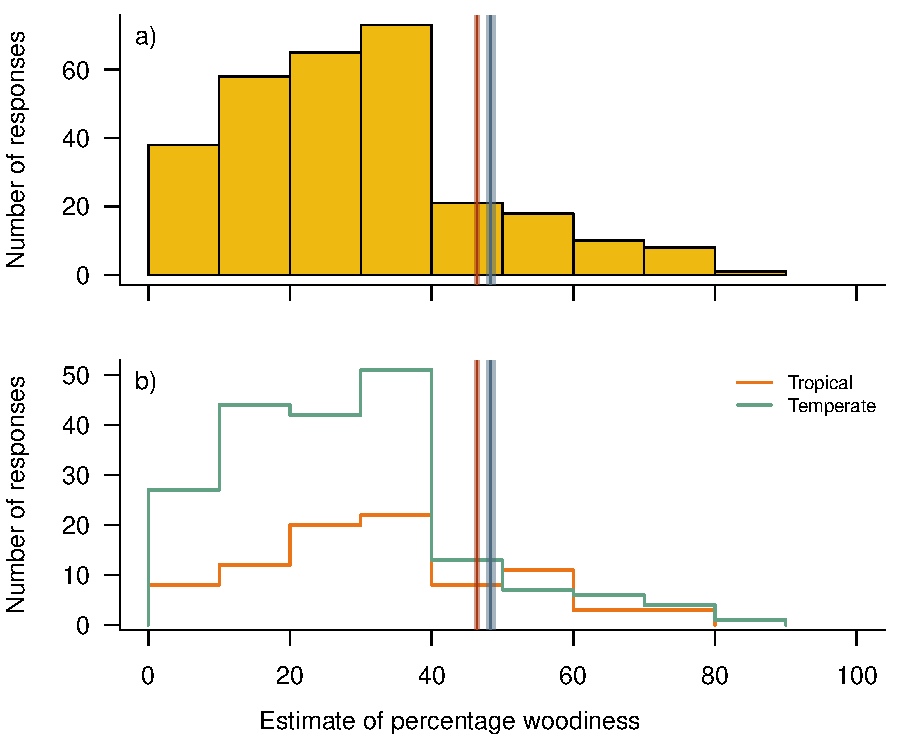
\includegraphics{figs/survey-distribution}
  \caption{(Supplementary) Distribution of all responses to the survey
    question ``What percentage of the world's vascular plant species
    are woody?''.
    %
    The mean and 95\% confidence intervals for our estimates of the
    proportion of woody species from the empirical data are depicted
    by the horizontal shaded rectangles; the blue rectangle
    corresponds to the ``weak prior'' approach and the red rectangle
    corresponds to the ``strong prior'' approach (see Appendix for
    details).  
    % 
    Panel A includes all 292 responses.  In panel B, the 282
    responses that indicated country are shown separated into
    ``tropical'' (orange distribution) and ``temperate'' (teal).
    Estimates from tropical countries were slightly, but
    significantly, higher than those from temperate countries
    ($p=$0.02, $r^2$=0.02).
  }

  \label{fig:survey-distribution}
\end{figure}

\begin{figure}[p]
  \centering
  \includegraphics{figs/fraction-on-phylogeny-supp}

  \caption{(Supplementary)
    \textit{This is Figure \ref{fig:phylogeny} using the alternative
      sampling approach.}\\
    %
    Distribution of the fraction of woodiness among orders of vascular
    plants.  Each tip represents an order, with the fraction of
    circumference proportional to the square root of the number of
    recognised species in that order (data from accepted names in
    \citet{ThePlantList}).  The bars around the perimeter indicate the
    percentage of woody (brown) and herbaceous (green) species,
    estimated using the ``weak prior'' (sampling with replacement)
    approach.  Using the ``strong prior'' approach generally leads to
    an estimated percentage that is further away from 50\% (see
    Figures \ref{fig:phylogeny} and \ref{fig:distribution-genera}).
    Phylogeny from \citep{Zanne}.  Orders not placed by APG-III
    \citep{APG3} are not displayed.}
  \label{fig:phylogeny-supp}
\end{figure}

\begin{figure}[p]
  \centering
  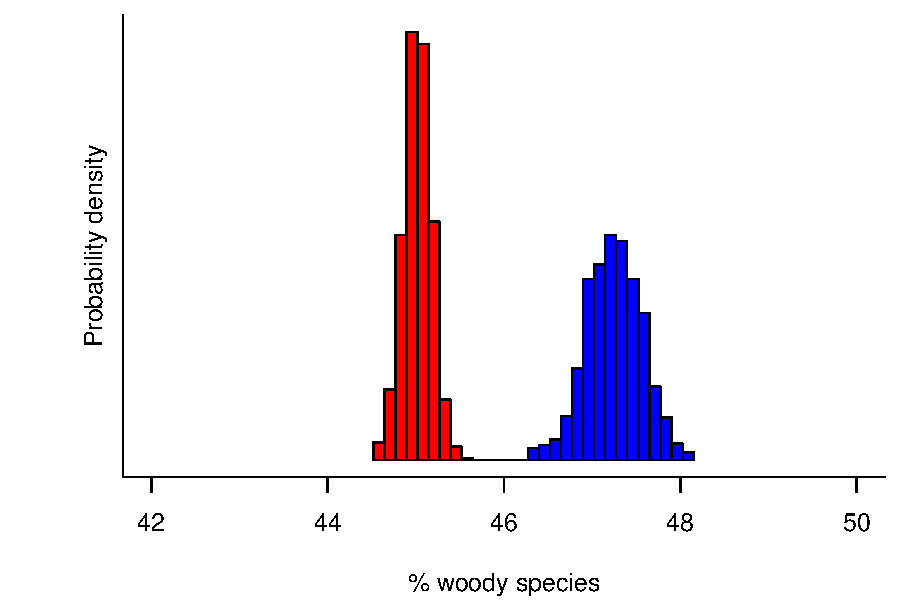
\includegraphics{figs/distribution-raw}  
  \caption{(Supplementary) The posterior probability distribution for
    the proportion of the world's flora that is woody, using our two
    sampling approaches.  The red (left) distribution samples missing species
    with replacement (strong prior), while the blue distribution
    (right) samples missing species without replacement (weak prior).
    See Appendix for details.}
  \label{fig:distribution-raw}
\end{figure}

\begin{table}[p]
  \centering
  \textit{[too large to set; see csv file]}
  \caption{Look-up table for converting the 103 growth form categories
    in the Royal Botanic Gardens Kew database into a binary
woody/herbaceous coding.}
\label{tab:kew}
\end{table}

\end{document}

%%% Local Variables:
%%% mode: latex
%%% TeX-master: t
%%% TeX-PDF-mode: t
%%% End:


